%  sample eprint article in LaTeX           --- M. Peskin, 9/7/00
%  modified for LHCP2014, Hong Ma hma@bnl.gov
%  This file is part of a tar file, which can be downloaded from the LHCP2014 indico site. 
%    https://indico.cern.ch/event/279518/
% 


\documentclass[10pt]{article}
\usepackage{graphicx}



%%%%%%%%%%%%%%%%%%%%%%%%%%%%%%%%%%%%%%%%%%%%%%%%%%%%%%%%%%%%%%%%%%%%%%%%%%%%
%   document style macros
%%%%%%%%%%%%%%%%%%%%%%%%%%%%%%%%%%%%%%%%%%%%%%%%%%%%%%%%%%%%%%%%%%%%%%%%%%%%
\def\Title#1{\begin{center} {\Large #1 } \end{center}}
\def\Author#1{\begin{center}{ \sc #1} \end{center}}
\def\Address#1{\begin{center}{ \it #1} \end{center}}
\def\andauth{\begin{center}{and} \end{center}}
\def\submit#1{\begin{center}Submitted to {\sl #1} \end{center}}
\newcommand\pubblock{\rightline{\begin{tabular}{l} Proceedings of the Second Annual LHCP\\ \pubnumber\\
         \pubdate  \end{tabular}}}

\newenvironment{Abstract}{\begin{quotation} \begin{center} 
             \large ABSTRACT \end{center}\bigskip 
      \begin{center}\begin{large}}{\end{large}\end{center} \end{quotation}}

\newenvironment{Presented}{\begin{quotation} \begin{center} 
             PRESENTED AT\end{center}\bigskip 
      \begin{center}\begin{large}}{\end{large}\end{center} \end{quotation}}

\def\Acknowledgements{\bigskip  \bigskip \begin{center} \begin{large}
             \bf ACKNOWLEDGEMENTS \end{large}\end{center}}
%%%%%%%%%%%%%%%%%%%%%%%%%%%%%%%%%%%%%%%%%%%%%%%%%%%%%%%%%%%%%%%%%%%%%%%%%%%%
%  personal abbreviations and macros
%    the following package contains macros used in this document:
\input econfmacros.tex
%%%%%%%%%%%%%%%%%%%%%%%%%%%%%%%%%%%%%%%%%%%%%%%%%%%%%%%%%%%%%%%%%%%%%%%%%%%

\textwidth=6.5in  \textheight=8.75in
\hoffset=-.85in
\voffset=-0.6in

%%  DO NOT CHANGE anything above.

% include packages you will need
\usepackage{color}
\usepackage{microtype}

%%%%%%%%%%%%%%%%%%%%%%%%%%%%%%%%%%%%%%%%%%%%%%%%%%%%%%%%%%%%%%%%%%%%
% basic data for the eprint:
%%%%%%%%%%%%%%%%%%%%%%%%%%%%%%%%%%%%%%%%%%%%%%%%%%%%%%%%%%%%%%%%%%%%

% Instruction:
% Please change each of the following fields:
%

%% preprint number data:
% If there is a preprint number from your institute, or experiment note number, please fill it in 
%\newcommand\pubnumber{ ATL-PHYS-PROC-2014-XXX }
\newcommand\pubnumber{ }

%% date
\newcommand\pubdate{\today}

%%  Affiliation
\def\affiliation{
On behalf of the CMS Experiment, \\
Department of Physics \\
University of Florida, Gainesville, FL, USA }

%% Acknowledge the support
\def\support{\footnote{Work supported by the US Department of Energy and National Science Foundation }}

\begin{document}

% large size for the first page
\large
\begin{titlepage}
\pubblock


%% Change the title, name, abstract
%% Title 
\vfill
\Title{ Search for the Standard Model Higgs Boson Decaying to $\mu^+\mu^-$ in $pp$ Collisions at $\sqrt{s}=7$ and 8 TeV with the CMS Detector }
\vfill

%  if you need to add the support use this, fill the \support definition above. 
%   \Author{ FIRSTNAME LASTNAME \support }
\Author{ Justin Hugon  }
\Address{\affiliation}
\vfill
\begin{Abstract}

A search for the standard model Higgs boson in the rare $\mu^+\mu^-$ decay channel is presented. The data samples, recorded by the CMS experiment at the LHC, correspond to integrated luminosities of $5.0\pm0.1$ fb$^{-1}$ at 7 TeV center-of-mass energy and of $19.7\pm0.5$ fb$^{-1}$ at 8 TeV. To enhance the Higgs signal over the dominant Drell-Yan background, the events are categorized by topologies corresponding to different production processes. Upper limits on the production rate, with respect to the Standard Model prediction, are reported at the 95\% confidence level for Higgs boson masses in the range from 120 to 150 GeV/c$^2$.

\end{Abstract}
\vfill

% DO NOT CHANGE 
\begin{Presented}
The Second Annual Conference\\
 on Large Hadron Collider Physics \\
Columbia University, New York, U.S.A \\ 
June 2-7, 2014
\end{Presented}
\vfill
\end{titlepage}
\def\thefootnote{\fnsymbol{footnote}}
\setcounter{footnote}{0}
%

% normal size for the rest
\normalsize 

%% Your paper should be entered below. 

\section{Introduction}

HERE IS YOUR INTRODUCTION, REPLACE THE TEXT

The program will be devoted to a review of the latest experimental and theoretical results on hadron collider physics and a discussion on the outlook for the coming years. The conference intends to provide a lively discussion between experimenters and theorists on topics such as the Standard Model Physics and Beyond, the Higgs Boson, Supersymmetry and Heavy Ion Physics and planning for the high luminosity upgrades.

\section{Observations}

REPLACE THE TEXT, FIGURE and TABLE.

Observation of the Higgs Boson,  \cite{Aad:2012tfa},\cite{Chatrchyan:2012ufa}. 

 
%%%%%%%%%%%%%%%%%%%%%%%%%%%%%%%%%%%%%%%%%%%%%%%%%%%%%%%%%%%%%%%%%%%%%%%%%
%%
%%   use this format to include an .eps figure into your paper
%%
\begin{figure}[htb]
\centering
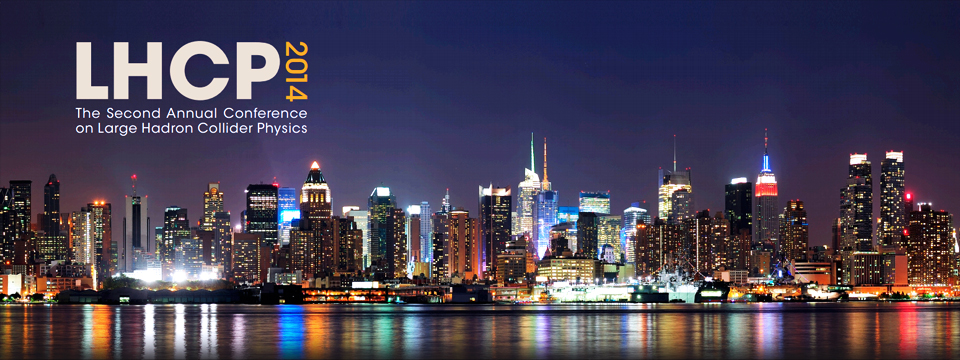
\includegraphics[height=2in]{head_lhcp2014.jpg}
\caption{ Place the caption here}
\label{fig:figure1}
\end{figure}
%%%%%%%%%%%%%%%%%%%%%%%%%%%%%%%%%%%%%%%%%%%%%%%%%%%%%%%%%%%%%%%%%%%%%%%%%%%

See Figure \ref{fig:figure1} and Table \ref{tab:table1}. 

%%%%%%%%%%%%%%%%%%%%%%%%%%%%%%%%%%%%%%%%%%%%%%%%%%%%%%%%%%%%%%%%%%%%%%%%%
%%
%%   use this format to include a LaTeX table  into your paper
%%
\begin{table}[t]
\begin{center}
\begin{tabular}{l|ccc}  
Patient &  Initial level($\mu$g/cc) &  w. Magnet &  
w. Magnet and Sound \\ \hline
 Guglielmo B.  &   0.12     &     0.10      &     0.001  \\
 Ferrando di N. &  0.15     &     0.11      &  $< 0.0005$ \\ \hline
\end{tabular}
\caption{ place the caption here }
\label{tab:table1}
\end{center}
\end{table}
%%%%%%%%%%%%%%%%%%%%%%%%%%%%%%%%%%%%%%%%%%%%%%%%%%%%%%%%%%%%%%%%%%%%%%%%%%%

\section{Interpretations}

The conference banquet will be hosted at the Spirit of New York, dinner while on a three-hour cruise around Manhattan. Enjoy an evening of most entertaining and unique combination of dining, dancing, entertainment and views on New York Harbor. Registered attendees and accompanying guests are invited to attend. 


\section{Conclusions}

...... 

%%  if necessary
\Acknowledgements
I am grateful to XYZ for fruitful discussions.


\begin{thebibliography}{99}

%%
%%  bibliographic items can be constructed using the LaTeX format in SPIRES:
%%    see    http://www.slac.stanford.edu/spires/hep/latex.html
%%  SPIRES will also supply the CITATION line information; please include it.
%%

%\cite{CMS:2013aga}
\bibitem{CMS:2013aga} 
  CMS Collaboration,
  ``Search for the standard model Higgs boson in the dimuon decay channel 
in pp collisions at sqrt(s)= 7 and 8 TeV,''
  CMS-PAS-HIG-13-007.
  %%CITATION = CMS-PAS-HIG-13-007;%%
  %9 citations counted in INSPIRE as of 24 Jul 2014

%\cite{CMS:yva}
\bibitem{CMS:yva} 
  CMS Collaboration,
  ``Combination of standard model Higgs boson searches and measurements of the properties of the new boson with a mass near 125 GeV,''
  CMS-PAS-HIG-13-005.
  %%CITATION = CMS-PAS-HIG-13-005;%%
  %302 citations counted in INSPIRE as of 24 Jul 2014

%\cite{CMS:2013xfa}
\bibitem{CMS:2013xfa} 
  CMS Collaboration,
  ``Projected Performance of an Upgraded CMS Detector at the LHC and HL-LHC: Contribution to the Snowmass Process,''
  arXiv:1307.7135.
  %%CITATION = ARXIV:1307.7135;%%
  %46 citations counted in INSPIRE as of 24 Jul 2014

\bibitem{Aad:2012tfa} 
  G.~Aad {\it et al.}  [ATLAS Collaboration],
  ``Observation of a new particle in the search for the Standard Model Higgs boson with the ATLAS detector at the LHC,''
  Phys.\ Lett.\ B {\bf 716}, 1 (2012)
  [arXiv:1207.7214 [hep-ex]].
  %%CITATION = ARXIV:1207.7214;%%
  %3009 citations counted in INSPIRE as of 22 Jul 2014
  
  
%\cite{Chatrchyan:2012ufa}
\bibitem{Chatrchyan:2012ufa} 
  S.~Chatrchyan {\it et al.}  [CMS Collaboration],
  ``Observation of a new boson at a mass of 125 GeV with the CMS experiment at the LHC,''
  Phys.\ Lett.\ B {\bf 716}, 30 (2012)
  [arXiv:1207.7235 [hep-ex]].
  %%CITATION = ARXIV:1207.7235;%%
  %2951 citations counted in INSPIRE as of 22 Jul 2014

%\cite{Chatrchyan:2013lba}
\bibitem{Chatrchyan:2013lba} 
  S.~Chatrchyan {\it et al.}  [CMS Collaboration],
  ``Observation of a new boson with mass near 125 GeV in pp collisions at $\sqrt{s}$ = 7 and 8 TeV,''
  JHEP {\bf 1306}, 081 (2013)
  [arXiv:1303.4571 [hep-ex]].
  %%CITATION = ARXIV:1303.4571;%%
  %188 citations counted in INSPIRE as of 24 Jul 2014

\end{thebibliography}

 
\end{document}

